\documentclass[]{jsarticle}
\usepackage[dvipdfmx]{graphicx}
\usepackage[deluxe]{otf}
\usepackage[hang,small,bf]{caption}
\usepackage[subrefformat=parens]{subcaption}
\captionsetup{compatibility=false}

\renewcommand{\kanjifamilydefault}{\mgdefault}
\newcommand*{\graphc}[3][7.0cm]{\begin{figure}[h] \begin{center}\includegraphics[clip,width= #1]{#2}\caption{#3}\end{center}\end{figure}}
% http://www.ai.soc.i.kyoto-u.ac.jp/~matsubara/le4-2016/index.php?%28Step1%29%20SVM%E3%81%AE%E4%BD%9C%E6%88%90


\begin{document}
\title{平成28年度 3回生後期実験(エージェント) \\ 課題2 SVMの評価 }
\author{村田 叡}
\date{ 2016/10/21 }
\maketitle

\section{プログラム概要}
前回の課題では 1 と -1 の2クラスのサンプル点集合を分類する識別器を生成した。
この課題ではそれの交差検定を行った。
ガウスカーネル または 多項式カーネルの最良パラメータを推定できるようになった。
以下にその詳細を述べる。

\section{外部仕様}

\subsection{svm.py}

今回のコードは 前回のコードの svm.py にて追加で実装した。
このコードは、引数としてサンプル点集合のファイル名、カーネル名、及びオプションをとる。
サンプル点集合の形式については、実験のページに書かれてあるものに従った。
カーネル名は、gauss, polynomial, sigmoid, linear のいずれかをとる。
デフォルトのカーネル名は gauss である。
--cross オプションを使うことで、交差検定ができる。
それのオプションに数字を指定することで、交差検定のデータの分割数を指定できる。
この交差検定は、ガウスカーネルまたは多項式カーネルについて適応できる。
指定しなかった場合は分割数は10である。
--plot オプションを使うと結果をプロットしたものをimagesフォルダに保存していく。


\subsection{実行例と実行結果}
\begin{verbatim}
# 必要なライブラリの導入
$pip3 install -r requirements.txt
# サンプル点集合 sample_circle.dat のガウスカーネルのSVMの交差検定をデータ分割数5で行う。
$python3 svm.py sample_circle.dat -m gauss -c 5
>> 2 ** -13.0000 : 67.0%
>> 2 ** -11.6000 : 67.0%
...
...
>> 2 ** -1.5060 : 96.0%
>> p : 0.34868591658760156 | 96.0%
\end{verbatim}
上記のように、徐々に範囲を狭めて適切な値を探索する。
最後の出力には適切なパラメータとその精度を表示する。


\section{内部仕様}
以下ではsvm.pyで、交差検定のために新たに実装した関数について述べる。

\subsection{cross\_validation(x,y,kernel,div)}
この関数では交差検定を行う。
引数は、サンプル点ベクトル集合 x,クラス集合 y,カーネル関数 kernel,分割数 div である。


\subsection{search\_parameter(x, y, kernel, param\_ranges, div, do\_plot=False, eps=0.001)}
この関数で、交差検定を用いることでパラメータを推定する。
引数は、サンプル点ベクトル集合 x,クラス集合 y,カーネル関数 kernel,
探索するパラメータの範囲 param\_ranges,分割数 div,
プロットするか否かの do\_plot,
探索を更に続けるかの eps をとる。
探索するパラメータの範囲は、 $i,offset$の2つのパラメータからなり、
$2^{i - offset} $ から $2^{ i + offset }$ の範囲を探す。
探索範囲をしぼめていって精度を上げていく。
eps を上げるほど、細部を探索しなくなる。


\section{考察}
以下では実際に上記のプログラムを用いて、分割数10の交差検定を行った予測精度の違いを述べる。
データは線形分離可能なデータと線形分離不可能なデータの2つについて、
カーネルはガウスカーネルと多項式カーネルの2つについてをそれぞれ述べる。
線形不可能なデータについては、やや湾曲した図形の自作のデータを用いた。
(画像を二値化して、実験データと同様のフォーマットのサンプルデータに変換するプログラム
image2scatter.py を書いてデータを作成した。(注: これの実行にはpillowが必要である))

\newpage
\subsection{ガウスカーネル}
ガウスカーネルは、パラメータ$\sigma$ に依存して、
$K(x_k,x_l) = exp(-||x_k-x_l||^2 / 2\sigma^2) $ と書ける。
下図のように、$\sigma$の値に応じて、教師の点の周りにのみ分類されやすくなるかどうかが変わる。
そういうカーネルなので、線形分離が可能な集合に対しては、本質的に弱点があるように思われる。

\begin{figure}[htbp]
 \begin{minipage}[b]{0.5\hsize}
  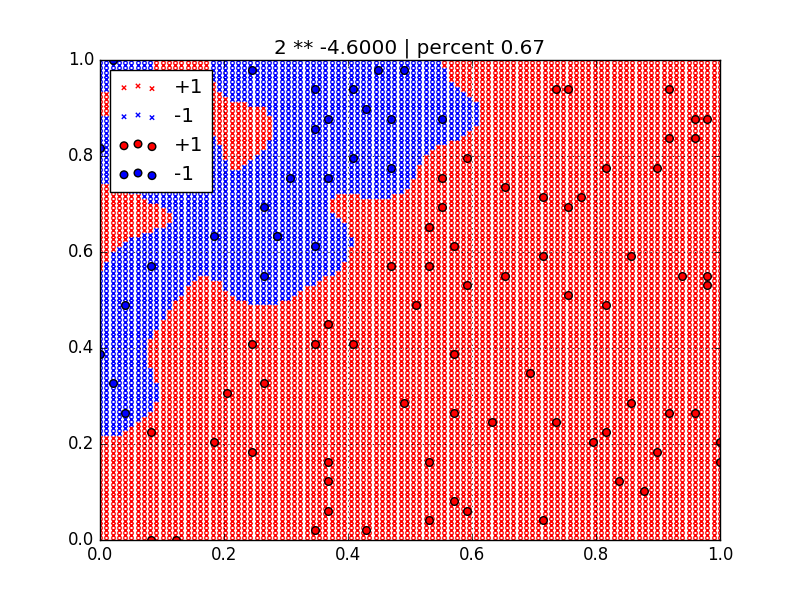
\includegraphics[scale=0.4]{./cross_validate_images/gauss_linears/1.png}
  \subcaption{精度67\% , $\sigma = 2^{-4.6}$}
 \end{minipage}
 \begin{minipage}[b]{0.5\hsize}
  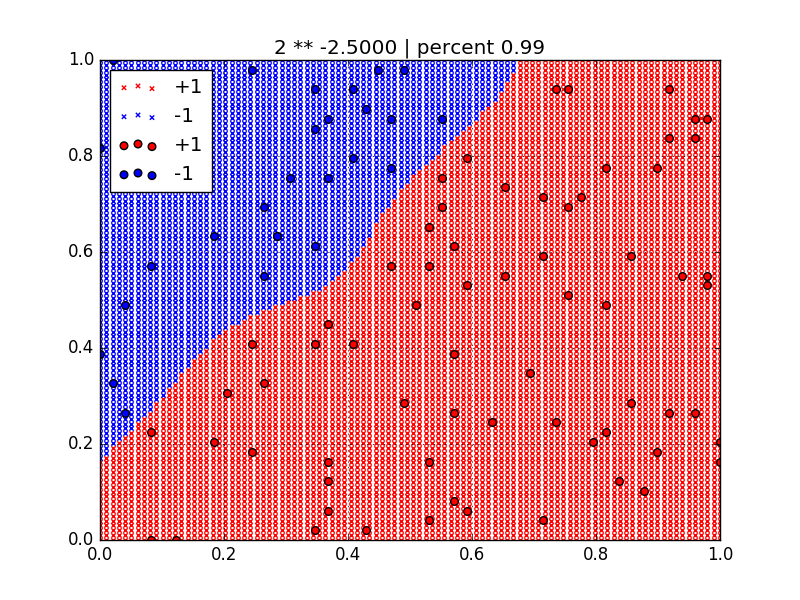
\includegraphics[scale=0.4]{./cross_validate_images/gauss_linears/2.png}
  \subcaption{精度99\% , $\sigma = 2^{-2.5}$}
 \end{minipage}
 \caption{線形分離可能習合のガウスカーネルの識別器}
\end{figure}

\begin{figure}[htbp]
 \begin{minipage}[b]{0.5\hsize}
  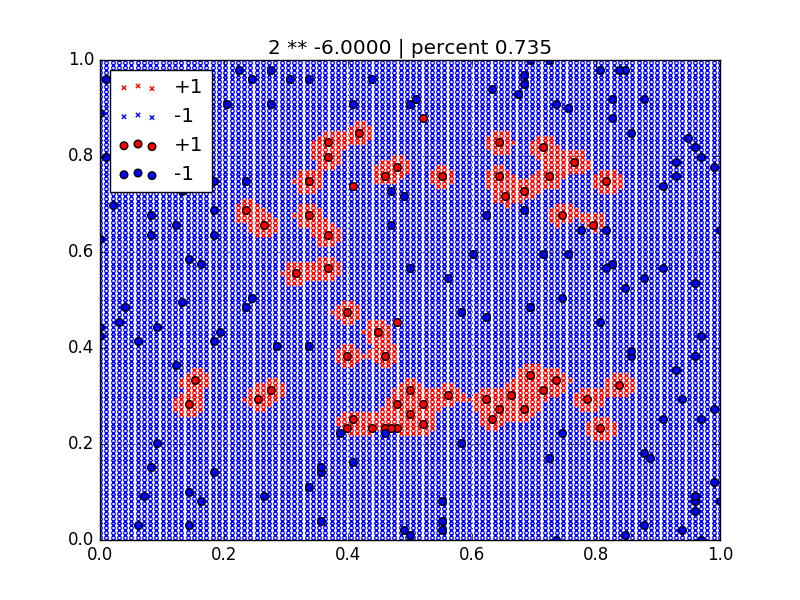
\includegraphics[scale=0.4]{./cross_validate_images/gauss_te/1.png}
  \subcaption{精度73.5\% , $\sigma = 2^{-6}$}
 \end{minipage}
 \begin{minipage}[b]{0.5\hsize}
  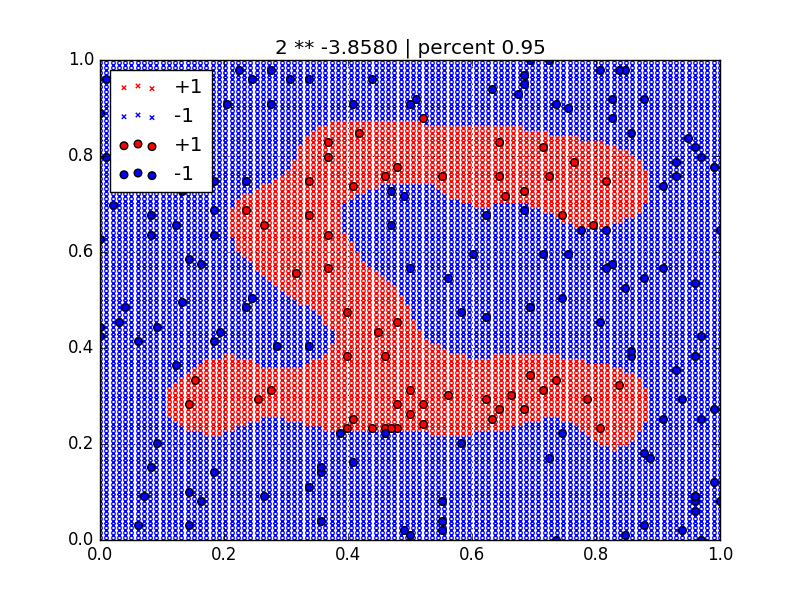
\includegraphics[scale=0.4]{./cross_validate_images/gauss_te/4.png}
  \subcaption{精度95\% , $\sigma = 2^{-3.858}$}
 \end{minipage}
 \caption{線形分離不可能習合のガウスカーネルの識別器}
\end{figure}

\newpage
\subsection{多項式カーネル}
多項式カーネルは、パラメータ$d$ に依存して、
$K(x_k,x_l) = (1+(x_k,x_l))^d $ と書ける。
ガウスカーネルと違って、教師の周りのサンプルをとるというよりは、
境界をなめらかに近似するように決定するように見える。
そういうカーネルなので、線形分離についてはサポートベクターも少なくて済み、
得意に見える。

\begin{figure}[htbp]
 \begin{minipage}[b]{0.5\hsize}
  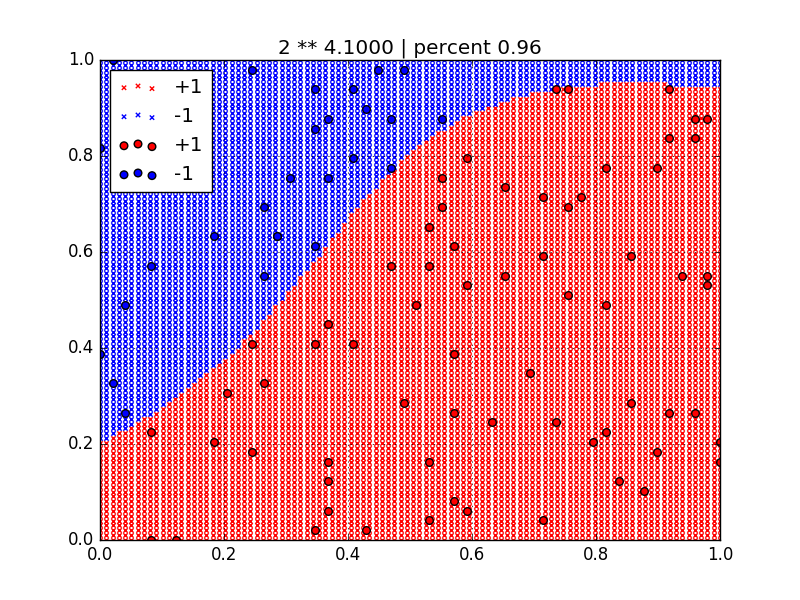
\includegraphics[scale=0.4]{./cross_validate_images/polym_linears/1.png}
  \subcaption{精度96\% , $d = 2^{4.1}$}
 \end{minipage}
 \begin{minipage}[b]{0.5\hsize}
  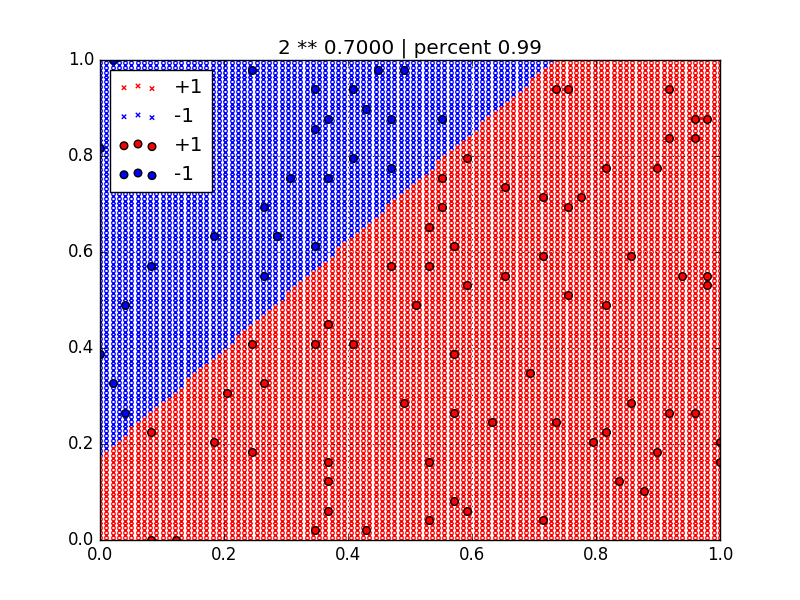
\includegraphics[scale=0.4]{./cross_validate_images/polym_linears/2.png}
  \subcaption{精度99\% , $d = 2^{0.7}$}
 \end{minipage}
 \caption{線形分離可能習合の多項式カーネルの識別器}
\end{figure}

\begin{figure}[htbp]
 \begin{minipage}[b]{0.5\hsize}
  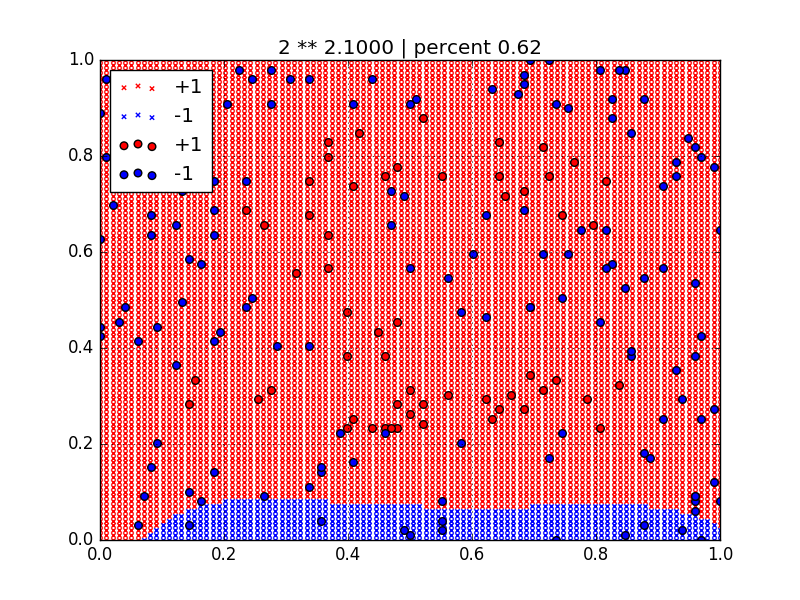
\includegraphics[scale=0.4]{./cross_validate_images/polym_te/1.png}
  \subcaption{精度62\% , $d = 2^{2.1}$}
 \end{minipage}
 \begin{minipage}[b]{0.5\hsize}
  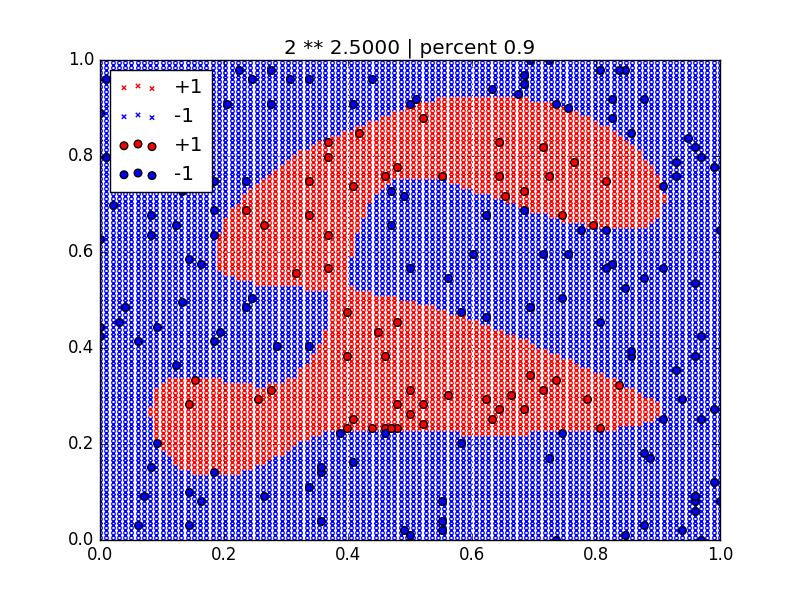
\includegraphics[scale=0.4]{./cross_validate_images/polym_te/2.png}
  \subcaption{精度90\% , $d = 2^{2.5}$}
 \end{minipage}
 \caption{線形分離不可能習合の多項式カーネルの識別器}
\end{figure}

\end{document}